\documentclass[a4paper,10pt]{article}
\usepackage{float}
\usepackage{graphicx}
\usepackage[utf8]{inputenc}
\usepackage[spanish]{babel}
\usepackage{listings}
\usepackage{hyperref}
\usepackage{enumitem}
\usepackage{bookmark}
\usepackage[nocolor]{drawstack}
\graphicspath{/imagenes,/Casos de prueba}

\title{		\textbf{Trabajo Práctico 1: \\
			Conjunto de instrucciones MIPS
			}}

\author{	Fabrizio Cozza, \textit{Padrón Nro. 97.402}                     \\
            \texttt{ fabrizio.cozza@gmail.com }                                              \\[2.5ex]
            Kevin Cajachuán, \textit{Padrón Nro. 98.725}                     \\
            \texttt{ kevincajachuan@hotmail.com }                                              \\[2.5ex]
            Luciano Giannotti, \textit{Padrón Nro. 97.215}                     \\
            \texttt{luciano\_giannotti@hotmail.com.ar}                                              \\[3.5ex]
	 \newline
            \normalsize{1er. Cuatrimestre de 2018}                                      \\
            \normalsize{66.20 Organización de Computadoras  $-$ Práctica Martes}  \\
            \normalsize{Facultad de Ingeniería, Universidad de Buenos Aires}            \\
       }
\date{}


\begin{document}
\maketitle
\thispagestyle{empty}   % quita el n�mero en la primer p�gina
\newpage

\section{Objetivos}

Este Trabajo Práctico tiene el fin de ayudarnos a familiarizarnos con el conjunto de instrucciones MIPS y el concepto de ABI, extendiendo un programa que resuelva el problema descripto en la siguiente sección.


\section{Programa}

El software de este trabajo está escrito en su mayoría en lenguaje C y permite dibujar \textbf{Julia Sets} o \textbf{Conjuntos de Julia} segun los parámetros que le pasamos por línea de comando.
Estos parámetros son la región del plano complejo: delimitada por un centro, un ancho y un alto; una semilla que afectará el calculo para cada pixel; la resolución y la salida ya sea por pantalla o por archivo. \\
La función en la cuál se encuentra la lógica de cómputo del fractal está escrita en MIPS con el fin de tener soporte nativo para NetBSD. \\
El formato a usar es  PGM o \textit{portable gray format}, que resulta útil para describir imágenes digitales en escala de grises.


\section{Implementación}

Una vez recibidos los parámetros, para dibujar el Julia Set el programa convierte cada píxel de la ventana a un punto en el plano complejo.
A ese punto se lo eleva al cuadrado y le suma la semilla mencionada en la sección anterior. Esto se repite hasta que el valor absoluto del resultado sea menor a 2, en cuyo caso se toma la cantidad de iteraciones y se imprime en el archivo PGM, representando el nivel de blanco de ese píxel.

\subsection{Funciones implementadas}
\subsubsection{mips32\_plot}
Esta función es la que se encarga de hacer los cálculos, para luego poder ir imprimiendo el valor de cada píxel en un archivo. \\
El único parámetro que recibe es un struct definido como \textit{param\_t} en el que se encuentran todos los datos necesarios para que la función realice su tarea, los cuales se obtienen de los parámetros pasados por el usuario por línea de comandos. \\
Esta función no devuelve nada ya que solo se dedica a hacer cálculos e imprimir. \\
El stack frame de esta función se muestra a continuación, en el cuál en cada dirección de memoria se indica qué variable está guardada.

\begin{center}
\begin{drawstack}
	\startframe
	\padding{1}{} \cellcom{60}
	\cell{ra} \cellcom{56}
	\cell{fp} \cellcom{52}
	\cell{gp} \cellcom{48}
	\finishframe{SRA}
	\startframe
	\cell{zi} \cellcom{44}
	\cell{zr} \cellcom{40}
	\cell{ci} \cellcom{36}
	\cell{cr} \cellcom{32}
	\finishframe{FRA}
	\startframe
	\cell{c} \cellcom{28}
	\cell{x} \cellcom{24}
	\cell{y} \cellcom{20}
	\cell{fd} \cellcom{16}
	\finishframe{LTA}
	\startframe
	\padding{1}{} \cellcom{12}
	\padding{1}{} \cellcom{8}
	\padding{1}{} \cellcom{4}
	\padding{1}{} \cellcom{0}
	\finishframe{ABA}
\end{drawstack}
\end{center}

\subsubsection{my\_fprintf}
Esta función imprime en un archivo llamando a la syscall \textit{write}, por lo que los parámetros que recibe son los mismo que recibe esta syscall: file descriptor del archivo, lo que se quiere escribir, y cuánto se quiere escribir. Finalmente devuelve la cantidad de bytes que se escribió la igual que la syscall. \\
El stack frame de esta función se muestra a continuación.

\begin{center}
\begin{drawstack}
	\startframe
	\padding{1}{} \cellcom{36}
	\cell{ra} \cellcom{32}
	\cell{fp} \cellcom{28}
	\cell{gp} \cellcom{24}
	\finishframe{SRA}
	\startframe
	\cell{total} \cellcom{20}
	\cell{n} \cellcom{16}
	\finishframe{LTA}
	\startframe
	\padding{1}{} \cellcom{12}
	\padding{1}{} \cellcom{8}
	\padding{1}{} \cellcom{4}
	\padding{1}{} \cellcom{0}
	\finishframe{ABA}
\end{drawstack}
\end{center}

\subsubsection{my\_strlen}
Esta función calcula la longitud de una cadena, recibiendo como parámetro la cadena y devolviendo la longitud. \\
El stack frame de la función se muestra a continuación. Al ser una función \textit{leaf}, no fue necesario tener un ABA ni salvar el registro \textit{ra}.
\begin{center}
\begin{drawstack}
	\startframe
	\cell{fp} \cellcom{4}
	\cell{gp} \cellcom{0}
	\finishframe{SRA}
\end{drawstack}
\end{center}

\subsubsection{int\_to\_str}
Esta función convierte un número a una cadena, llamando para realizar esto a dos funciones: \textit{dig\_to\_char} y \textit{put\_end}. Lo único que recibe la función es el número que se quiere convertir y no devuelve nada. \\
El stack frame se muestra a continuación.

\begin{center}
\begin{drawstack}
	\startframe
	\padding{1}{} \cellcom{36}
	\cell{ra} \cellcom{32}
	\cell{fp} \cellcom{28}
	\cell{gp} \cellcom{24}
	\finishframe{SRA}
	\startframe
	\cell{index} \cellcom{20}
	\cell{number} \cellcom{16}
	\finishframe{LTA}
	\startframe
	\padding{1}{} \cellcom{12}
	\padding{1}{} \cellcom{8}
	\padding{1}{} \cellcom{4}
	\padding{1}{} \cellcom{0}
	\finishframe{ABA}
\end{drawstack}
\end{center}

\subsubsection{dig\_to\_char}
Esta función recibe un número que se quiere convertir a cadena, un array para ir guardando los caracteres de cada dígito del número y el índice actual en el que hay que ir guardando cada caracter. Esta función se llama recursivamente para ir obteniendo los dígitos del número e ir guardandolos en el array. Como esto es lo único que realiza, la función no devuelve nada. \\
A continuación se muestra el stack frame de esta función.

\begin{center}
\begin{drawstack}
	\startframe
	\padding{1}{} \cellcom{36}
	\cell{ra} \cellcom{32}
	\cell{fp} \cellcom{28}
	\cell{gp} \cellcom{24}
	\finishframe{SRA}
	\startframe
	\padding{1}{} \cellcom{20}
	\cell{r} \cellcom{16}
	\finishframe{LTA}
	\startframe
	\padding{1}{} \cellcom{12}
	\padding{1}{} \cellcom{8}
	\padding{1}{} \cellcom{4}
	\padding{1}{} \cellcom{0}
	\finishframe{ABA}
\end{drawstack}
\end{center}

\subsubsection{put\_end}
Esta función lo único que hace es poner el caracter \textbackslash0 al final del array en que se guardaron los dígitos del número, para poder imprimirlo más adelante. Por esta razón esta función recibe como parámetros el array y el índice en el que se tiene que guardar el caracter \textbackslash0 y no devuelve ningún valor. \\
El stack frame se muestra a continuación. Por la misma razón que en la función \textit{my\_strlen}, no es necesario tener un ABA ni salvar \textit{ra}.

\begin{center}
\begin{drawstack}
	\startframe
	\cell{fp} \cellcom{4}
	\cell{gp} \cellcom{0}
	\finishframe{SRA}
\end{drawstack}
\end{center}
%\section{Pruebas}
%
%Para las pruebas compilamos el programa con gcc de la siguiente manera:
%
%\begin{lstlisting}[frame=single]
%$gcc main.c -o tp0
%\end{lstlisting}
%Luego corremos el archivo \textbf{test.sh}.
%Ya que las pruebas son sobre las imágenes, las vamos a realizar a ojo comparandolas con las del enunciado y con las obtenidas en un generador online (\url{http://usefuljs.net/fractals/}).
%
%Cabe destacar que las imagenes del generador tienen mayor rango dinamico que las del enunciado y nosotros decidimos generarlas como en \'{e}ste \'{u}ltimo.
%
%Las imagenes obtenidas por nuestro trabajo se encuentran tambi\'{e}n en formato PNG en la subcarpeta \textit{imagenes}.
%A su vez las imagenes del generador online se encuentran en \textit{Casos de prueba}.
%
%\subsection{Caso con los valores por defecto}
%Se obtiene una imagen como la primera figura del enunciado:
%
%\begin{lstlisting}[frame=single]
%$./tp0 -o uno.pgm
%\end{lstlisting}
%
%\begin{figure}[H]
%\begin{center}
%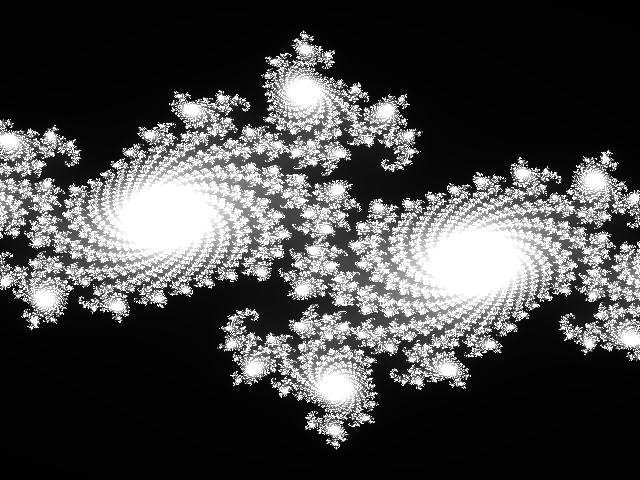
\includegraphics[width=0.5\textwidth]{imagenes/uno.png}
%\caption{} \label{uno}
%\end{center}
%\end{figure}
%
%\newpage
%
%\subsection{Caso de imagen con zoom y otro centro}
%Se obtiene una imagen como la segunda figura del enunciado:
%
%\begin{lstlisting}[frame=single]
%$ ./tp0 -c 0.282-0.007i -w 0.005 -H 0.005 -o dos.pgm
%\end{lstlisting}
%
%\begin{figure}[H]
%\begin{center}
%
\includegraphics[width=0.5\textwidth]{imagenes/dos.png}
%\caption{} \label{dos}
%\end{center}
%\end{figure}
%
%\subsection{Caso de imagen con ancho 1 y centro 1}
%Se obtiene una imagen como la primera del enunciado pero con un zoom x2 aplicado:
%
%\begin{lstlisting}[frame=single]
%$ ./tp0 -w 1 -H 1 -o tres.pgm
%\end{lstlisting}
%
%\begin{figure}[H]
%\begin{center}
%
\includegraphics[width=0.5\textwidth]{imagenes/tres.png}
%\caption{} \label{tres}
%\end{center}
%\end{figure}
%
%\newpage
%
%\subsection{Caso de imagen muy chica}
%
%Imprimimos una imagen de 8x6 para que se puedan notar claramente los pixeles en la pantalla.
%
%\begin{lstlisting}[frame=single]
%$ ./tp0 -r 8x6 -o cuatro.pgm
%\end{lstlisting}
%
%\begin{figure}[H]
%\begin{center}
%
\includegraphics[width=0.5\textwidth]{imagenes/cuatro.png}
%\caption{} \label{cuatro}
%\end{center}
%\end{figure}
%
%\subsection{Caso de imagen con otra semilla}
%
%Esta imagen usa una semilla con sus dos componentes negativas y la imaginaria mucho mas grande que la real.
%\begin{lstlisting}[frame=single]
%$ ./tp0 -s -0.157-1.041i -o cinco.pgm
%\end{lstlisting}
%
%\begin{figure}[H]
%\begin{center}
%
\includegraphics[width=0.5\textwidth]{imagenes/cinco.png}
%\caption{} \label{cinco}
%\end{center}
%\end{figure}
%
%\newpage
%
%\subsection{Caso de imagen muy angosta}
%En este caso cambiamos la resolucion para obtener una imagen de un pixel
%de alto y 800 de ancho. \newline
%Es dif\'{i}cil observarla en el informe por lo que decidimos no colocarla. Sin embargo el archivo se encuentra en la misma carpeta del TP con el nombre \textit{seis.pgm}.
%
%\begin{lstlisting}[frame=single]
%$ ./tp0 -r 800x1 -o seis.pgm
%\end{lstlisting}

\section{Código S}

En esta sección se muestra el código 

\lstinputlisting[basicstyle=\ttfamily\scriptsize,breaklines=true]{../mips32_plot.S}

\section{Bibliografía}
\begin{enumerate}
\item GXemul. \\ http://gavare.se/gxemul/.
\item The NetBSD project. \\
	http://www.netbsd.org/.
\item Conjunto de Julia \\ 
	http://es.wikipedia.org/wiki/Conjunto\_de\_Julia (Wikipedia).
\item PGM format specification.\\
	http://netpbm.sourceforge.net/doc/pgm.html.
\item Generador de fractales. \\
	http://usefuljs.net/fractals/
\item GIMP. \\
	https://www.gimp.org/
\item System V Application Binary Interface. \\
	http://math-atlas.sourceforge.net/devel/assembly/mipsabi32.pdf
\end{enumerate}

\end{document}